\section{Dictionary Learning}
\begin{description}
    \item[Fixed Orthonormal Basis] $\ $
        \begin{figure}[H]
            \centering
            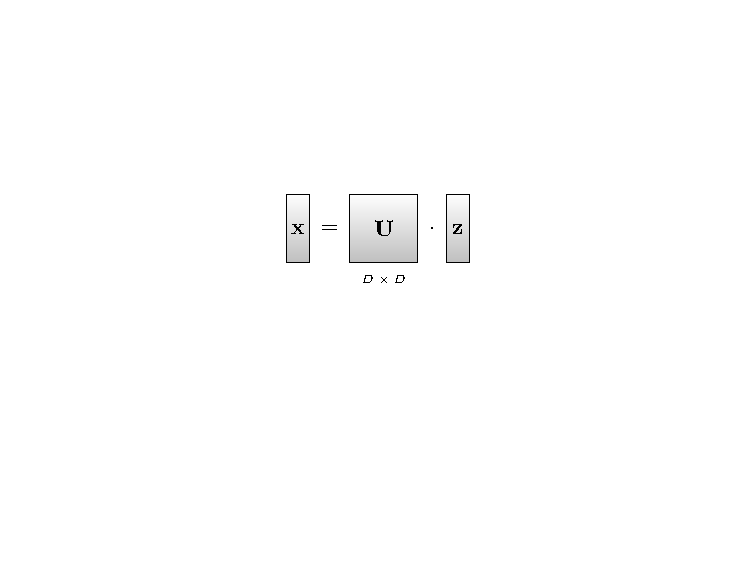
\includegraphics[width=0.5\textwidth,page=1]{img/10_bases}
        \end{figure}
        \subitem Advantage: Efficient coding by matrix multiplication $z = U^Tx$.
        \subitem Disadvantage: Only sparse for a single class of signals.

    \item[Fixed Overcomplete Basis] $\ $
        \begin{figure}[H]
            \centering
            \includegraphics[width=0.5\textwidth,page=2]{img/10_bases}
        \end{figure}
        \subitem Advantage: Sparse coding for several signal classes.
        \subitem Disadvantage: Finding the sparsest code
            \begin{itemize}
            \item Requires an approximation algorithm,
            \item Is problematic if the dictionary size is $L$ and the coherence $m(U)$ is large.
            \end{itemize}

    \item[Learning the Dictionary] $\ $
        \subitem Advantage: We adapt the dictionary to signal characteristics and thus get the same approximation error achievable with a smaller $L$.
        \subitem Disadvantage: We have to solve a matrix factorisation problem. 
        \begin{figure}[H]
            \centering
            \includegraphics[width=0.7\textwidth,page=3]{img/10_bases}
        \end{figure}
        subject to sparsity constraint on $Z$ and atom norm constraint on $U$.
\end{description}

\subsubsection{Matrix Factorisation}
\begin{align*}
    (U^*, Z^*) \in \argmin_{U,Z} \norm{X-U\cdot Z}_F^2
\end{align*}
We observe that the objective function is \emph{not convex} in both $U$ and $Z$ (local minima). But convex in either $U$ or $Z$ (unique minimum).
\paragraph{Iterative Greedy Minimisation} $\ $
\begin{enumerate}
    \item Initialisation
    
        The minimisation is sensitive to the choice of $U^0$: The initial candidate solution is optimised locally and greedily until no progress is possible.
        \begin{description}
            \item \emph{Random atoms}:
            
                Sample $\{u_l^0\}$ on the unit sphere:
                \begin{enumerate}
                    \item Sample $D$ dimensional standard normal distribution:
                        \begin{align*}
                             u_l^0 \sim \mathcal N (0,ID).
                        \end{align*}
                    \item Scale to unit length:
                        \begin{align*}
                            u_l^0 \gets {u_l^0 \over  \norm{u_l^0}_2}.
                        \end{align*}
                \end{enumerate}
            \item \emph{Samples from $X$}:
                \begin{enumerate}
                    \item $u_l^0\gets x_n$, where $n\sim \mathcal U(1,N)$ is sampled uniformly.
                    \item Scale to unit length:
                        \begin{align*}
                            u_l^0 \gets {u_l^0 \over  \norm{u_l^0}_2}.
                        \end{align*}
                \end{enumerate}
        \end{description}
        Use \emph{fixed overcomplete dictionary}, e.g. overcomplte DCT.
    \item Coding step:
        \begin{align*}
             Z^{t+1} \in \argmin_Z \norm{X-U^t\cdot Z}_F^2,
        \end{align*}
        subject to $Z$ being sparse and fixed $U$.
        
        Since each column is separable we get:
        \begin{align*}
            \norm{R}_F^2 = \sum_{i,j} r_{i,j}^2 = \sum_j \norm{r_j}_2^2.
        \end{align*}
        Thus we obtain $N$ \emph{independent} sparse coding steps:
        \begin{align*}
            z_n^{t+1} &\in \argmin_z \norm{z}_0,
            \text{s.t. }\ &\norm{x_n}
        \end{align*}


    \item Dictionary update step:
        \begin{align*}
            U^{t+1} \in \argmin_U \norm{X-U\cdot Z}_F^2,
        \end{align*}
        subject to $\norm{u_l}_2 - 1\ \forall l\in[1,L]$ and fixed $Z$.
        
        In contrast to the coding step the residual is \emph{not separable} in atoms (columns of $U$).
        
        \emph{Approximation}: Update on atom at a time. $\forall l\in[1,L]$:
        \begin{enumerate}
            \item Set $U = [u_1\ldots u_l\ldots u_L^t]$ fix for all atoms except $u_l$.
            \item Isolate $R_l^t$ that minimises $R_l^t$ subject to $\norm{u_l^*}_2 =1$.
                \begin{align*}
                    &\norm{X-[u_1^t\ldots u_l \ldots u_L^t]\cdot Z^{t+1}}_F^2\\
                    =&\norm{
                        X-\left(
                                \sum_{e\neq l} u_e^t (z_e^{t+1})^T + u_l (z_l^{t+1})^T
                            \right) 
                    }_F^2\\
                    =& \norm{R_l^t - u_l (z_l^{t+1})^T}_F^2,
                \end{align*}
                where $z_l^T$ is the $l$-th row of matrix $Z$.
            \item Find $u_l^*$ that minimises $R_l^t$, subject to $\norm{u_l^*}_2 = 1$.
                
                We observe that $u_l(z_l^{t+1})^T$ is an outer product, i.e. a matrix.
                Hence we need to minimise the residual
                \begin{align*}
                    \norm{R_l^t - u_l (z_l^{t+1})^T}_F^2
                \end{align*}
                by approximating $R_l^t$ with a rank-1 $u_l (z_l^{t+1})^T$.
                
                This is achieved by SVD of $R_l^t$:
                \begin{align*}
                    R_l^t = \tilde U S\tilde V^T = \sum_i s_i \tilde u_i \tilde v_i^T,
                \end{align*}
                $u_l^* = \tilde u_1$ being the first left-singular vector. 
                
                We also observe that $\norm{u_l^*} =1$ is naturally satisfied.
        \end{enumerate}
\end{enumerate}








































